
\documentclass[11pt]{article}
\title{Unicef User Testing Task Form}
\author{Matteo Sissa, Lorenzo Prosch, Annachiara, Ivan Della Vecchia}

\usepackage{hyperref}
\usepackage{geometry}
\usepackage[]{eforms}
\usepackage{graphicx}

\geometry{
	top=2cm,
	right=2cm,
	left=2cm,
	bottom=2cm
}



\begin{document}
	\maketitle
	\renewcommand{\arraystretch}{3.5}
	
	\vspace{0.5cm}
	
	\begin{Form}
		
		\begin{tabular}{p{10cm} p{10cm}}
			
			\TextField[width=4cm, bordercolor=]{Nome: } &
			\TextField[width=4cm, bordercolor=]{Cognome: }\\
			\ChoiceMenu[combo, name=countryField, bordercolor=, width=5cm]{Età: }{20, 21, 22, 23, 24, 25, 26, 27, 28, 29, 30} &
			\TextField[width=3cm, bordercolor=, format={dd/mm/yyyy}]{Data: }\\
			
		\end{tabular}
		
		\vspace{1cm}
		
		\subsection*{Lista dei Task}
		\begin{enumerate}
			
			\item Unicef è impegnata in molti problemi umanitari e tra questi vi sono temi rilevanti come l'uguaglianza di genere, la nutrizione (in particolare la nutrizione infantile), il cambiamento climatico, la risposta al COVID-19...\\ Per ogni importante area di interesse per Unicef, il sito web offre innanzitutto una \textbf{pagina di alto livello} con una panoramica del lavoro che Unicef sta svolgendo in tale ambito. Successivamente, all'interno di queste pagine di alto livello, l'utente può trovare \textbf{risorse} (articoli, report...) che approfondiscono ulteriormente il tema generale\\
			A titolo di esempio, il sito web di Unicef offre una pagina dedicata alla questione dei bambini con disabilità e all'interno di questa pagina di alto livello è possibile individuare risorse relative all'argomento che sono visualizzate con la seguente grafica:
			\begin{center}
				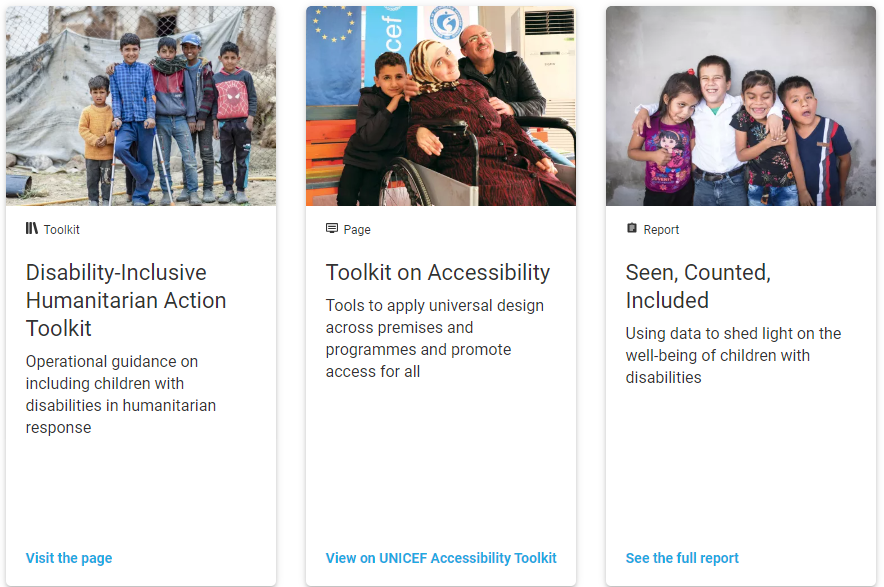
\includegraphics[width=0.6\linewidth]{res/Resources}
			\end{center}
			
			
			Il primo compito consiste nel familiarizzare con queste pagine di presentazione sul sito web. Quindi, supponiamo che tu fossi interessato al tema dell'\textbf{uguaglianza di genere}, riesci a individuare la pagina web che fornisce una panoramica del lavoro che Unicef sta svolgendo in quell'ambito? Una volta lì, sei in grado di elencare \textbf{TUTTE} le \textbf{risorse} relative all'uguaglianza di genere?
			Ora, prova a ripetere la stessa procedura anche per gli argomenti della \textbf{risposta al COVID-19} e della \textbf{nutrizione}.
			
			
			\item Unicef raggiunge molti dei suoi obiettivi anche grazie alle generose \textbf{donazioni} di persone provenienti da tutto il mondo che credono nei principi e nelle idee dell'organizzazione. Di conseguenza, una delle azioni più rilevanti che un utente può compiere sul sito web ufficiale di Unicef è quella di effettuare una donazione per una delle cause presentate sulla pagina. Per testare questa funzionalità, supponiamo di voler donare a Unicef per sostenere specificamente \textbf{l'emergenza in Afghanistan} (quindi \textit{NON} una donazione generale a Unicef), riesci a trovare l'area corretta del sito web per svolgere questo compito?
			
			\item Unicef opera in molti paesi diversi del mondo con scopi e obiettivi diversi. Di conseguenza, il sito web è strutturato in modo tale che vi siano sottopagine dedicate a ciascun paese specifico in cui Unicef opera. Supponiamo che tu fossi interessato a leggere specificamente cosa sta facendo o organizzando Unicef in Italia, riesci a trovare la pagina web di \textbf{Unicef Italia} navigando da quella principale?
			
			\item \textit{The State of the World's Children} è un rapporto annuale che Unicef pubblica per illustrare le minacce più rilevanti nel mondo contemporaneo alla sopravvivenza dei bambini. È il fiore all'occhiello dell'organizzazione, quindi è estremamente importante. Supponiamo che tu volessi trovare questo rapporto per \textbf{l'anno 2023}, nel quale viene spiegato e illustrato il problema della vaccinazione dei bambini. Sei in grado di individuarlo e scoprire \textbf{le quattro soluzioni} che Unicef propone per \textbf{vaccinare} il maggior numero possibile di bambini contro le malattie e le patologie più pericolose per la vita?\\
			N.B. \textit{Non} è necessario scaricare l'intero report, la pagina di presentazione del rapporto è sufficiente.
			
			\item Oltre a donare denaro, un modo alternativo per contribuire alle cause di Unicef è collaborare come \textbf{stagista} in una delle aziende partner o direttamente in Unicef. Il sito web dovrebbe essere in grado di attrarre stagisti da tutto il mondo e rendere il processo di candidatura il più semplice possibile. Ora supponiamo che tu stessi navigando sul sito web per trovare \textbf{opportunità di lavoro} per uno stage, sei in grado di individuare la sezione corretta del sito web da esaminare e elencare tutte le opportunità di stage offerte nello stato del \textbf{Sudafrica} (South Africa)?\\
			N.B. Stage è "internship" in inglese.
			
			\item Per ogni argomento sul sito web di Unicef ci sono molti articoli correlati che vengono mostrati e l'utente è in grado di sfogliarli e leggere ciò che gli interessa. Questo task consiste nel trovare un articolo specifico sul sito di Unicef, senza conoscere in anticipo la sua posizione esatta. Quindi, supponiamo che tu fossi interessato a leggere un articolo sulla \textbf{situazione della vaccinazione COVID-19 in Bangladesh}. Il titolo dell'articolo è nello specifico \textit{Bangladesh's COVID-19 vaccination rate has soared in a year}. Sei in grado di navigare intuitivamente dalla homepage del sito web di Unicef alla posizione corretta dove potrebbe essere collocato questo articolo?
			
			
		\end{enumerate}
		
		
		
	\end{Form}
	
	
	
\end{document}